\chapter{Hydrogel design for protein separation}\label{ch03}
\section{How we made the hydrogels}
We made hydrogels with anchored fragments of FG Nups.  We started with a precursor solution in an aqueous buffer containing the protein fragment, monomers and crosslinkers, and either a chemical initiator or photoinitiator.  Upon crosslinking, one end of the Nup fragment was anchored into the gel and the other left free, like the situation in the nuclear pore.

We used two major types of hydrogel: PEG and acrylamide.  The PEG hydrogels were made with 20 kD 8-armed PEG-norbornene, a PEG dithiol crosslinker, and either lithium phenyl-2,4,6-trimethylbenzoylphosphinate (LAP) \cite{fairbanks09} or 1-[4-(2-hydroxyethoxy)-phenyl]-2-hydroxy-2-methyl-1-propane-1-one (sold as Irgacure 2959) %http://www.xtgchem.cn/upload/20110629045632.PDF
as photoinitiators.  The acrylamide hydrogels were made in an aqueous buffer with dilutions of a 30\% solution of acrylamide and bis-acrylamide (29:1) ratio, the Nup fragment, and either a chemical initiator system (ammonium persulfate and TEMED) or LAP.

In order to crosslink the Nups into the hydrogel, we added a terminal cysteine to the Nups.  In the case of the PEG hydrogels, a Michael-thiol `click' reaction took place between the cysteine and norbornene upon crosslinking \cite{chatani14}.  For the acrylamide gels, another step was necessary.  I conjugated bisacrylamide to the cysteines using the reaction that Ben told us about with triethanolamine.  Then the bis-labeled Nups were able to link into the hydrogel when the precursor was crosslinked.

When a photoinitiator was used, we crosslinked the gels with UV light.  We used either a UV LED (look up typical intensity at gel plane from logbook) or a 405 laser on a confocal microscope.  Depending on the situation, we used photomasks to selectively expose regions of precursor to UV, or crosslinked entire droplets of precursor solution.  After crosslinking, hydrogels were rinsed with 10-100 times their volume with buffer and allowed to soak in fresh buffer solution overnight at 4$^\circ$C in order to approach swelling equilibrium and remove any remaining precursor solution.

Following the buffer soak, typically a fluorescent solution of proteins was added to the gels.  Usually this consisted of a transport factor (typically NTF2) and a similarly-sized inert protein (typically the red fluorescent protein mCherry).  A typical experiment consisted of a video at 4x or 10x magnification the hydrogel, reservoir chamber, and (if applicable) an outlet/inner reservoir which slowly accumulated protein as it passed through the gel.  Experiments ranged from 1-24 hours, with 2 hours being the most common.  Typical data produced was a plot of accumulation in the inner reservoir or hydrogel over the course of the experiment, as well as a concentration profile through the gel and inner reservoir.

\section{Microfluidic flow chambers}
Most experiments took place in microfluidic flow chambers.  These were typically 70-500 $\mu$m thick and consisted of a plastic (acrylic?) slide with ports drilled into it and a glass coverslip, separated by a spacer made of double-stick tape, cured Norland Optical Adhesive (NOA), or polydimethylsiloxane (PDMS).  The precursor solution was pipetted into the chamber and masked, or a drop was placed into the the chamber before it was sealed.  After crosslinking, the chamber was filled with buffer as described above.

Many different types of chamber were tried, and I will put in a picture of some of them.  The double-stick tape chambers are thin (70 $\mu$m per tape layer), of reliable thickness, and quick to make.  However, they often leak or dry overnight.  NOA ``sticker'' chambers are watertight and durable but they are difficult to make and to reuse \cite{paustian13}.  Chambers made with PDMS gaskets are thicker (100-400 $\mu$m) and their thickness is not as reproducible, but they are easy to reuse, often can last several days without drying out, and are quick to assemble.  Likewise, if liquid needs to be flowed through a chamber, short lengths of PEEK tubing can be glued into the ports and fitted with Tygon tubing.  For sufficiently gentle flows, however, ports can be left simply as holes in the plastic slide and pipette tips inserted.  Most of the chambers are thin enough that liquid wicks easily through to the other port(s).

NOA stickers were made following the methods in \cite{paustian13}.  First, a template was created in the Silhouette craft cutter software.  The craft cutter was used to cut this template into a layer of packing tape on a glass slide.  The unwanted tape was carefully peeled away, and the slide used as the basis for a PDMS mold.  Finally, a drop of NOA (usually 81, sometimes 61) was placed on the mold and covered with a coverslip.  The system was crosslinked using the UV LED for 3 seconds, at which point all but a thin surface layer of NOA was crosslinked on the coverslip.  The layer at the glass-PDMS boundary is slower to cure because of the presence of oxygen.  The sticker was carefully removed from the PDMS mold and positioned on the plastic slide with ports.  The slide and coverslip were exposed to UV for one minute to finish the curing process, and then rinsed with ethanol (to remove any uncured NOA) and water.  This process leaves a thin layer of NOA on the coverslip inside the chamber.  If that is not desired (and we have some evidence that proteins stick to the NOA layer), the coverslip can be pressed onto the clean PDMS mold and NOA slowly wicked in around the chamber.

PDMS gaskets were made by calculating the volume of PDMS mixture needed to make a layer of a specific thickness in a petri dish and then crosslinked at 70$^\circ$ and cut into shape with a razor.  Plasma-cleaning was tried in order to bond the PDMS to the glass, but it didn't work very well and ultimately the PDMS formed an adequate seal if cleaned with ethanol (as long as the chamber was not subjected to high pressures).  Silanation of the glass slides was also tried in order to bond the hydrogel more securely to the slide, but that didn't work and wasn't needed.  The gels bonded well as long as they were in place before crosslinking.  After crosslinking, they didn't stick to the chambers very well.

We also tried making very thin chambers for fluoresence recovery after photobleaching (FRAP) using the confocal microscope.  To make these chambers, we placed coverslips on glass slides (both carefully cleaned with ethanol and dried with house air) with 6-$\mu$m diameter beads as spacers.  A drop of hydrogel was crosslinked in the chamber and fluorescent protein solution wicked in.  The chamber was sealed with valap (a 1:1:1 ratio of vaseline, lanolin, and paraffin which easily melts over a burner and re-solidifies rapidly).  This didn't really work for FRAP, but thicker chambers did (see the next chapter).

Sometimes thick PDMS chambers were used to hold larger gels.  A 5-mm thick PDMS gasket chamber with port-less slides sealed to the top and bottom typically lasts at least a few weeks without drying.  Wrapping the chambers in saran wrap also helps prevent drying.  A flat thick piece of PDMS should be sealed over the ports to prevent drying.

\section{Hydrogel geometries}
Ideally, we wanted to test protein separation by looking at selective passage of transport factors through a hydrogel and into an outlet reservoir.  We tried several different hydrogel geometries in an effort to realize this setup.  I'll put in a picture of many of these.

We made a chamber in an x-shape with a port at the end of each arm and made a gel at the junction.  Then one side was filled with fluorescent proteins and the other with buffer.  We could watch the proteins move through the gel and into the outlet side.  Unfortunately, the outlet is large enough that accumulation was not noticeable, and it was of variable volume.  These chambers are also tricky to make and dry out rapidly.

Another chamber design featured an outlet reservoir much smaller than the inlet, with no ports in the outlet.  A bar of hydrogel was made to separate the inlet and outlet (using photomasks) and then soaked in buffer for 24 hours to remove all excess precursor solution from the outlet.  Then the inlet was filled with fluorescent proteins and their influx into the gel as well as through the gel into the outlet was monitored.  This setup allowed us to see the entire outlet at once and measure its volume.  The volume was also small enough to allow for fairly rapid equilibration.  On the downside, it took a long time to be sure that all of the precursor solution had diffused out of the outlet before starting the experiment, and there is a strong possibility that we were unknowingly crosslinking the outlet lightly.  We made a lot of these gels but they were not reproducible enough.

One slight variation on the small-outlet gets was the filled-outlet gel.  It used the same chamber, but we crosslinked the entire outlet.  This was an attempt to model a semi-infinite slab of gel.

We also made gels in a ring shape with an inner reservoir.  See the section on confocal crosslinking for a detailed description. Katie made some ring gels that were a few millimeters across with a PDMS mold.  These would have been optimal for selectivity but we couldn't work out the logistical problems (again, see section on confocal crosslinking).  The problem with using the molds to make rings is that they don't seal well to chambers if they're put into the chambers after being crosslinked, even when they are squished into the chambers.

Finally, we made gels out of single droplets of precursor solution squished into the chamber before crosslinking.  These have volumes of 0.5-2 $\mu$L.  These gels cannot be used to monitor selective transport through and exit from the gel, but we can use them to measure the diffusion constants of proteins within the gel and the selective influx of transport factors.  These gels have the advantage that they are easy to make and have much less severe edge effects than the gels made with a photomask.  The experimental chapter deals entirely with this type of hydrogel, which was typically made in a 400 $\mu$m PDMS gasket chamber with two PEEK-less ports.

\section{Pore size}

One of the biggest problems we faced was that of pore size.  Although there is a range of pore sizes in any hydrogel, and it's not actually always obvious how to define it, we wanted an average pore size large enough that we could be confident that any differences in the behavior of transport factor and inert protein were due to their interactions with the Nups, not slight differences in size or interactions with the hydrogel.  At the same time, we wanted the anchored Nups to fill a significant portion of the pore.  This meant that we wanted a hydrogel with pores somewhere between 10 and 20 nm on average.  It turns out that this is a difficult regime for hydrogels.  It's easy to get pores signicantly smaller using acrylamide or PEG systems, or significantly larger using systems like collagen, but the intermediate regime is difficult.  We tried many methods of increasing the pore size of our PEG and acrylamide hydrogels, including changing the composition and crosslinker, as well as adding porogens.  Finally, we settled on 6\% acrylamide hydrogels as being reasonably good for NTF2 and mCherry comparisons (both proteins are about 30 kD and we probably couldn't have used any larger ones in these gels).  This remained a source of frustration throughout the experiments.

I tried to calculate average pore size using an equation which I will cite here.  Most people use the swelling ratio or microrheology to determine pore size, which is difficult for us because the hydrogels are not very reproducible and they are also very small.  I used a paper which does not rely on those measurements, but also is probably not very accurate.  My estimate was that the average pore size in a 10\% wt PEG hydrogel is about 5 nm, which is roughly the same size as NTF2 and mCherry.  This means that we were likely seeing a lot of interactions/hindrance by the gel in the PEG gel experiments.  We were unable to lower the PEG or crosslinker concentration significantly without going below the gel point and being unable to make gels.

We did attempt to fix the problem with the PEG hydrogels by moving to a longer crosslinker.  We switched from a 1 kD to an 8 kD PEG dithiol linker.  The longer linker made the hydrogels swell more and be more porous at equilibrium, but it also made the gels softer and less mechanically stable.  Overall, the decrease in stability outweighed the improved pore size.  We also tried using non-PEG crosslinkers, including a coiled-coil protein (cite here) and DNA.  We could never get the coiled-coil protein to express, and the DNA crosslinker didn't form a gel.  We also tried putting a cysteine at each end of the Nup and using it as a crosslinker, but that didn't form a gel either.

Finally, we switched to acrylamide gels because the pore size was slightly better and the mechanical properties better.  I think acrylamide has a more heterogeneous pore structure than PEG, which we decided was a good thing.  Entry into the 6\% acrylamide gels was consistent and similar for NTF2 and mCherry.  I will put in a figure of some kind here.

\section{Porogens}

I tried to make gels with a larger pore size by using porogens.  These are nanoscale particles that can be mixed into the gel precursor solution and then removed/dissolved after crosslinking.  The idea is that then they would leave pores of a better size and also make it easier for the gel to swell to equilibrium.  I tried alginate nanospheres (which could then be removed by chelating the calcium ions) and large molecular-weight dextrans that could be removed by digesting with dextranase.  Neither of these options worked out.  I couldn't get the nanospheres to reliably resuspend in the precusor solution.  The dextran/dextranase system was more promising, but too much dextran remained in the hydrogels even after dextranase digestion.  Also the dextranase chewed up the FSFG.

\subsection{Alginate nanospheres}
% LKM book 5, pgs 26-36
\begin{figure}
\caption{Alginate crosslinking from \cite{bruchet15}. Alginate is composed of alternating guluronate (G) and mannuronate (M) blocks.  Addition of calcium ions leads to an ``egg-box'' crosslinked structure. Add a cartoon of spheres in our gel (with positive poly-L-lysine coating around negative alginate gel) and the spaces they should leave upon depolymerization.}
\centering
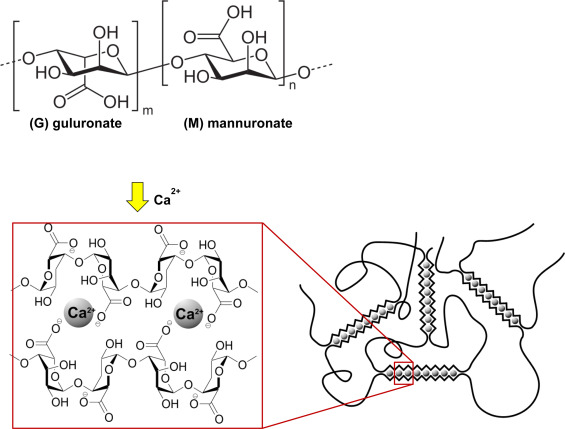
\includegraphics[width=0.5\textwidth]{figs/ch03/alginate-crosslinking}
\label{fig:alginate}
\end{figure}
Alginate is a monomer that can be made to polymerize by adding calcium ions (or other divalent ions?).  Include a picture of the alginate structure with and without calcium.  It's inert (and edible) and the polymerization can be reversed by adding EDTA or another chelating agent to remove the calcium.  Alginate salts are available in a number of average molecular weights and viscosities.

A number of protocols exist for creating alginate microspheres, but fewer are appropriate for nanospheres, which is the scale that we would need in order to use them as a porogen.  I did make spheres following the method described in \cite{de03}.

I prepared 10 mL of 0.6 mg/mL alginic acid sodium salt (Sigma, low-viscosity, product number A0628) in water.  Even a small amount of sodium alginate added to water creates a viscous solution that takes a lot of time and stirring to dissolve.  I used the Garcea lab sonicator with the microtip at 40\% amplitude to sonicate the sodium alginate solution while adding 2 mL of 0.67 mg/mL calcium chloride in water drop-by-drop.  I then stirred the solution on a magnetic stir plate for 30 minutes before adding 2 mL of 0.3 mg/mL poly-L-lysine in water.  The solution was stirred 30 more minutes before finally being spun down (check spinning conditions in lab book).

I tested several methods of preparing the nanospheres for addition to the hydrogel precursor solution.  First, the nanospheres were left in the solution in which they were made.  Second, the nanospheres were spun down out of that solution at 14400g for 10 minutes and immediately resuspended in deionized water.  (The pellet becomes more difficult to resuspend if it is not immediately resuspended.) Finally, the nanospheres were lyophilized and resuspended in water.  The resuspended solution remained cloudy even after several days, and so I didn't pursue lyophilizing the nanospheres.

The radius and diffusion coefficients of the both the non-spun and spun nanospheres were determined using a Titan DynaPro dynamic light scattering (DLS) system.  The non-spun nanospheres had an average radius of 170 $\pm$ 10 nm, with an estimated diffusion constant of 1.1~$\pm$~0.1~$\mu$m$^2$/s.  The nanospheres that had been spun and resuspended had two populations: almost entirely particles of radius 210~$\pm$~10~nm and diffusion constant 1.05~$\pm$~0.06~$\mu$m$^2$/s, and a small number of very large particles.  The large particles are probably aggregates from centrifugation.

After measuring the size distribution of the two samples, I added EDTA in an effort to depolymerize the nanospheres.  The maximum final EDTA concentration was 25~mM, and the samples were left to sit up to 30 minutes.  Re-running the DLS data gave inconclusive results as to the presence or size of remaining particles.  The fits did not change much, although the large aggregates appeared to have vanished from the spun sample.  It appeared that at least some nanospheres remained.

Next, the nanospheres were added to hydrogel precursor solution, which was then crosslinked.  Several nanosphere concentrations were tested before a condition was found in which the nanospheres appeared by eye to resuspend.  An approximately 2 $\mu$L nanosphere pellet (spun down from 10 mL of solution) was resuspended in a final concentration of 0.11 mg/mL PEG-ene, 0.09 mg/mL 8K PEG dithiol linker, and 5 mM LAP, all in 50 mM MOPS buffer pH 7.4.  The MOPS buffer was chosen because it has no divalent cations (and thus will not interfere with the alginate nanospheres).  The isoelectric point of poly-L-lysine is at about pH 5, and the nanospheres should be kept above that pH so their coating remains intact.

However, even these gels were clearly inhomogeneous under 4x magnification.  In an attempt to depolymerize the nanospheres, the resulting hydrogels were rinsed with PTB pH 5 (to remove any possible poly-L-lysine coating) and then soaked in 100~mM EDTA for two days.  No change was observed under 4x magnification.  For comparison, a macroscopic alginate droplet dissolved after 20 minutes in 100 mM EDTA and vortexing.  New gels were made and soaked in a pH 5 buffer (to remove any poly-L-lysine coating) and then in a solution containing 100 mM EDTA and 200 mM sodium citrate.  Gels remained cloudy and no change was observed.

Given the difficulty in resuspending and depolymerizing the alginate nanospheres, our focus shifted to developing a dextran/dextranase porogen system.

\subsection{Dextran/dextranase porogen system}
% First proof of concept: LKM book 5 pgs. 37-47
% add diagram of porogen process + molecular structure of dextran, dextranase?
Following the alginate nanospheres attempt, we tried creating nanopores using high-molecular-weight (high-MW) dextran.  Dextran is a branched, inert polymer that is commerically available at molecular weights up to 250 kD.  We used two sizes as porogens, 70 kD ($R_H \approx 10$ nm) and 250 kD ($R_H \approx 15$ nm) \cite{masuelli13}.  

As a proof of concept, I made and crosslinked precursor solutions containing 100~$\mu$M 70~kD dextran-rhodamine or 250~kD dextran-fluorescein.  The precursor contained 12\% acrylamide and 3.3\% bisacrylamide in 50~mM sodium acetate (NaOAc) buffer pH~5 as well as 2~mM LAP.  The precursor solution was crosslinked as 1-$\mu$L hydrogels in a 400-$\mu$m tall PDMS gasket chamber for 20~s using the UV LED.  After rinsing with NaOAc buffer, the chamber was filled with a freshly-made solution of 20~mg/mL dextranase (Sigma, D5884, dextranase from \textit{Penicillium sp.}) in NaOAc buffer.  Chamber was immediately placed in the Olympus widefield's environmental chamber, held at 37$^\circ$C, and imaged overnight. The fluorescence intensity in the dextranase-treated gels decreased significantly more rapidly than that of gels which contained dextran but were not treated with dextranase (Fig.~\ref{fig:dxase-equilibration}).  In the case of 70~kD dextran, the fluorescence reached a steady value (equilibrated, same as that in the reservoir) in approximately 100 minutes, while the non-treated case wasn't equilibrated after an overnight incubation.  For the 250~kD dextran, both the treated and non-treated gels reached an equilibrium in approximately the same amount of time, but the treated gel equilibrated much closer to the reservoir level than the non-treated gel.  Both sets of gels indicate that dextranase is able to digest the dextran within the hydrogels, allowing a significant amount of dextran and digest products to leave the gel, as expected.
\begin{figure}
\caption{Exit of fluorescent dextran from hydrogels after digestion with dextranase.}
\centering
\includegraphics[width=\textwidth]{figs/ch03/dxase-equilibration}
\label{fig:dxase-equilibration}
\end{figure}
% dextranase gels from 1/24/18; control gels from 1/22/18
% I also seem to have a replicate from 3/6/18

The next step in attempting this porogen system was recreating the effect in FSFG gels.  Unfortunately, it became clear that the dextranase was digesting the FSFG as well as the dextran (Fig.~\ref{fig:dxase-FSFG}).  
\begin{figure} % gel is from 6/19/18
\caption{Dextranase digestion of FSFG}
\centering
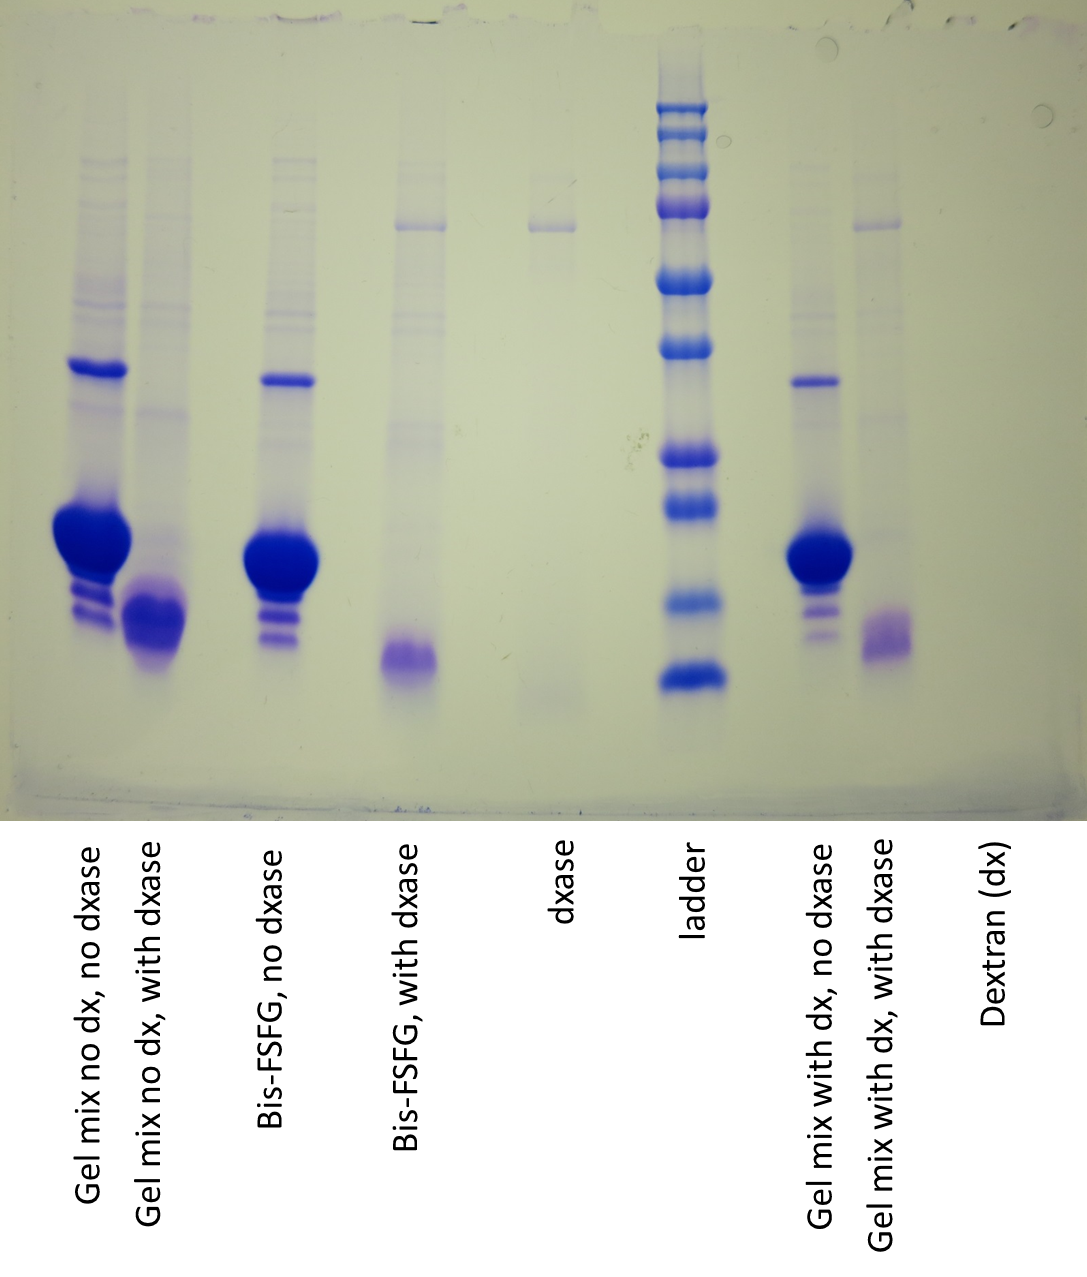
\includegraphics[width=0.5\textwidth]{figs/ch03/180619_LKM_dx+FSFG}
\label{fig:dxase-FSFG}
\end{figure}
 At this point, we stopped trying to use the dextran-dextranase porogen system for FSFG gels.  However, we did investigate the effect of dextran-dextranase treatment on the pore size in acrylamide hydrogels without anchored proteins.  Contrary to expectations, dextran-dextranase treatment did not increase subsequent diffusion of fluorescent proteins into the treated hydrogels.  For these experiments, I used 200~kD non-fluorescent dextran in the acrylamide precursor solution.  After the gels (either 12\% or 6\% final acrylamide concentration) were crosslinked, I treated them with 20~mg/mL dextranase solution in sodium acetate buffer (freshly made solution) for 2 hours at 37$^\circ$C in an incubator.  Then I rinsed the gels with buffer and let them sit in fresh buffer in the fridge overnight.  (Check this - sometimes I used a syringe pump to flow 10~mL of PTB through overnight, instead of letting the chamber sit.) The next day, I challenged the gels with a solution containing 10~$\mu$M each IgG-Alexa488 (150~kD) and mCherry (28~kD).  I monitored the accumulation of each protein in the gel over time (Fig.~\ref{fig:dxase-results}).  In both the 12\% and 6\% acrylamide gels, dextran-dextranase treatment did not improve influx of IgG-Alexa488 over corresponding non-treated gels.  In 6\% acrylamide gels, the influx of mCherry also remained approximately the same for treated and non-treated gels.  This indicates that dextran-dextranase treatment does not significantly increase the pore size in acrylamide hydrogels.  This is probably because significant dextran remains in the gel even after dextranase treatment, as suggested by Fig.~\ref{fig:dxase-equilibration}.
\begin{figure}
\caption{Accumulation of fluorescent proteins in gels treated with dextranase.}
\centering
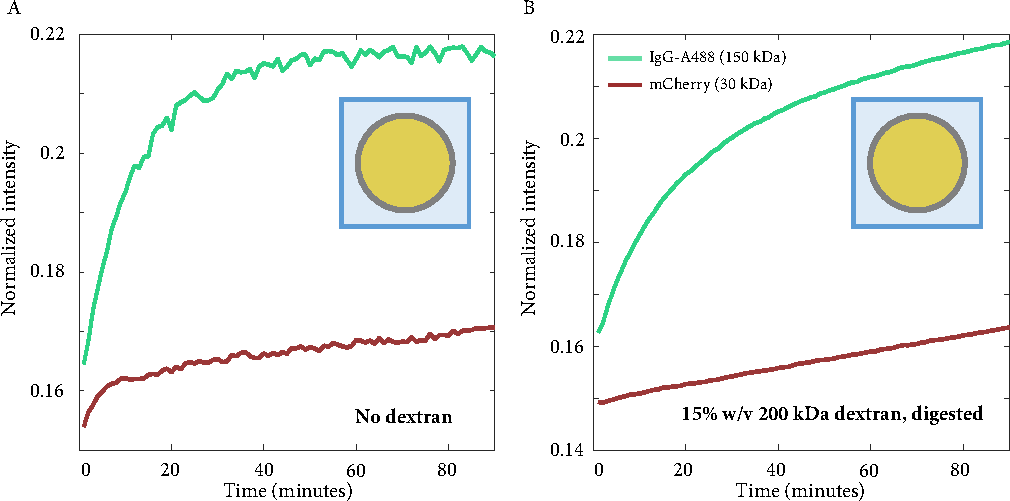
\includegraphics[width=\textwidth]{figs/ch03/dxase-results}
\label{fig:dxase-results}
\end{figure}
Unusually, the 12\% acrylamide gels showed an odd effect with mCherry accumulation.  In two separate instances, dextranase treatment appeared to suppress the entry of mCherry into both the dextran-containing hydrogel and the no-dextran control gel in the same chamber (Fig.~{fig:mCherry-suppression}).  IgG-Alexa488 accumulation remained the same as a non-treated gel.  Tests of gels without dextran but treated with dextranase did not show this mCherry suppression.  I didn't thoroughly investigate this effect.  The only thing I can think of that's different between the gels that did and didn't show mCherry suppression is that the gels that suppressed mCherry were in the presence of both dextran and dextranase, and therefore also dextran digestion products (which are mostly maltose, I believe).  Maybe the presence of maltose (despite the fact that it should have been thoroughly rinsed away) interfered with the accumulation of mCherry.  It's odd.
\begin{figure}
\caption{Suppression of mCherry in control gels that were in the presence of dextranase, dextran, and dextran digestion products (maltose).}
\centering
\includegraphics[width=\textwidth]{figs/ch03/mCherry-suppression}
\label{fig:mCherry-suppression}
\end{figure}
In conclusion, dextranase is capable of digesting a significant fraction of high-MW dextran within an acrylamide hydrogel.  However, a significant amount of the dextran still remains in the gel even after an overnight rinse, meaning that dextran-dextranase treatment does not result in noticeably larger pores overall.  In addition, the dextranase we used digested the FSFG peptide as well as dextran.  Dextran-dextranase treatment is not suitable as a porogen system for our hydrogels.

\section{Polymerization using confocal microscope}
 Make a cartoon figure explaining confocal setup and Bowman lab setup.

Given the problems that arose using photomasks and a UV LED to make hydrogels, I tested a crosslinking method using a 405 nm laser on the Nikon A1R spinning disc confocal microscope in the JSCBB microscopy facility.  Once a region of interest has been defined with the Nikon software, the photobleaching setting can be used to selectively expose regions of the field of view to UV light.  The precursor solution therefore crosslinks in the region of interest only.  This method is similar to that used in \cite{paustian13}, but the masking is done using the A1R software instead of a physical mask in the back focal plane.

I was able to ``draw'' hydrogels of arbitrary shapes using the 10x objective on the confocal along with the 405 nm laser at 100\% power.  Figure~\ref{fig:LW-gel-images} shows hollow rings with an outer diameter of about 600 $\mu$m and an inner diameter of 500 $\mu$m, as well as lines with a width of about 50 $\mu$m.  In order to crosslink the precursor solution, two raster-scans of the laser across the region of interest were needed, with the longest-allowable dwell time per pixel.  (In the microscope settings, the shortest dwell time is set as `1' and the longest as `1/32'.)  The precursor solution contained 0.5 mM LAP, 110 mg/mL 20kD 8-armed PEG-norbornene, 11 mg/mL 1kD PEG-dithiol, and 1 mM TCEP in PTB; it was used to fill 70-$\mu$m-thick sticky-tape or NOA flow chambers.

% hydrogel recipes on LKM book 4 pg 47, 56

Crosslinking with the confocal has several advantages over LED crosslinking.  Significantly smaller features are possible using the confocal.  50-$\mu$m features are consistent and reproducible, and features down to approximately 25 $\mu$m are possible, in contrast with the effective 100-$\mu$m lower limit using the LED and photomasks.  Additionally, arbitrary shapes, including shapes with inner cavities, are possible using the confocal.  Multiple small hydrogels can be created in the same chamber, including hydrogels of varying composition, created by removing the excess precursor solution and refilling the chamber with a different solution.  Finally, the degree of crosslinking can potentially be varied by changing the photobleaching settings.

\begin{figure} % LKM book 4 pg 81 (rings), LKM book 4 pg 77 (lines)
\caption{Image of laser-written ring control hydrogels. 9/6/16, and FSFG-A647 lines 8/25/16}
\centering
%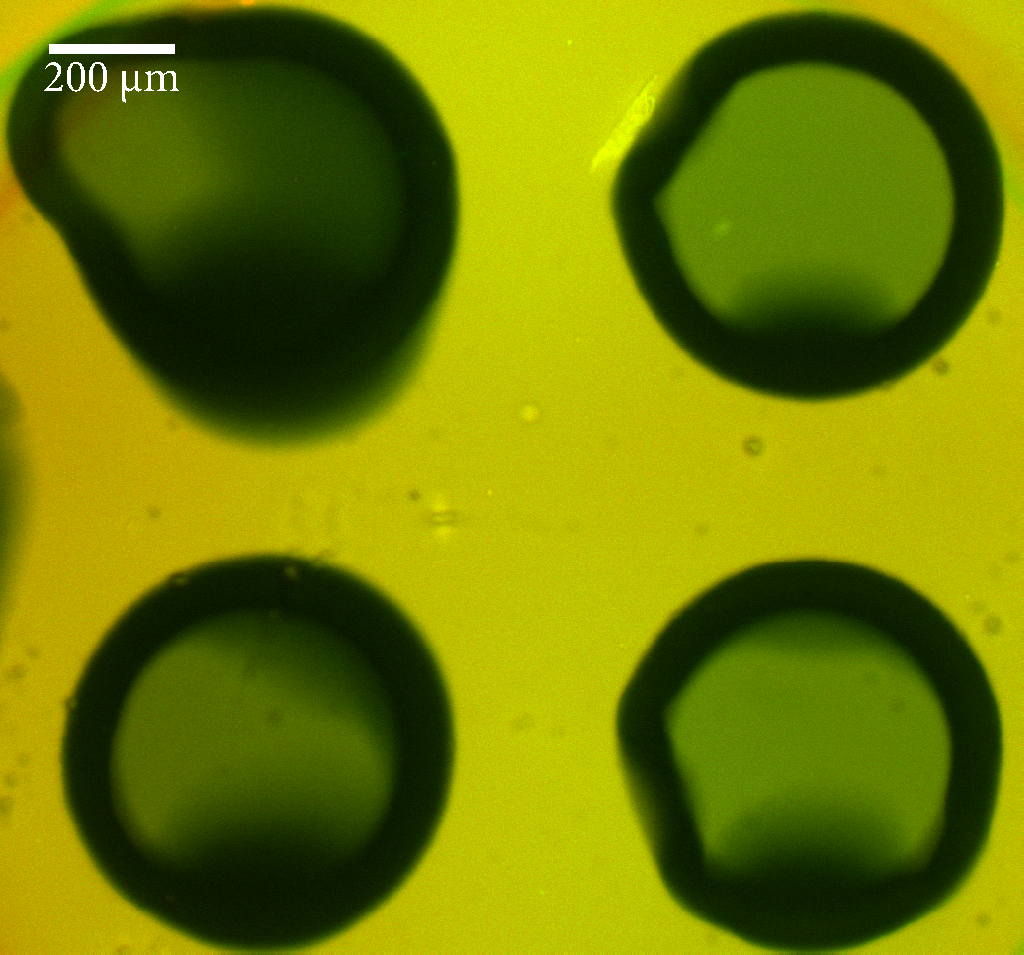
\includegraphics[width=0.5\textwidth]{figs/ch03/160906_laserGelImage_200umscale.pdf}
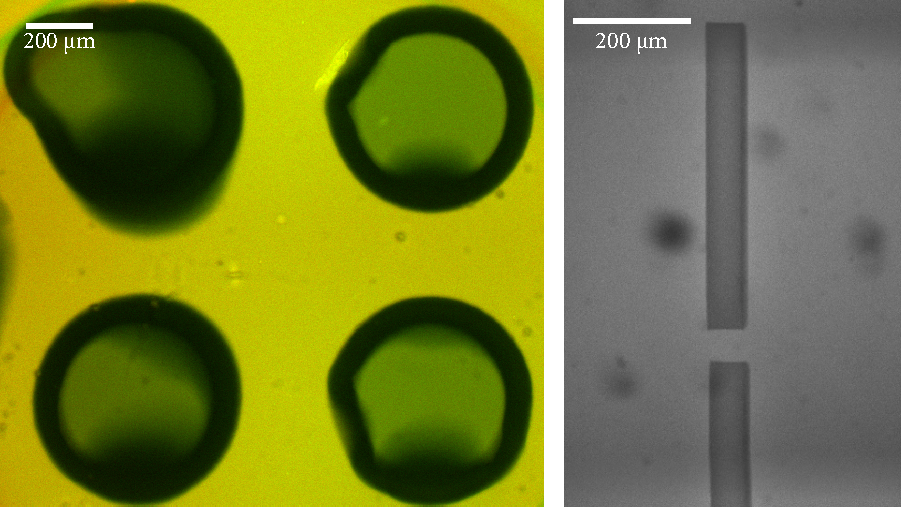
\includegraphics[width=0.7\textwidth]{figs/ch03/example-LW-gels}
\label{fig:LW-gel-images}
\end{figure} % microscope settings for rings: 1/32 dwell, 2 loops, 100% photobleaching intensity, nominal outer diameter = 600 um, nominal inner diameter = 500 um

The most appealing geometry made possible with confocal crosslinking is the hydrogel ring, as shown in Figs.~\ref{fig:LW-gel-images} and \ref{fig:LW-NTF2-images}.  Unlike all other hydrogel-chamber geometries, the inner reservoir is small enough to equilibrate in only a few hours (Fig.~\ref{fig:ring-acc-and-profile}).  Ideally, the hydrogel rings could have been used to test selective flux through the NPC mimics, a possibility not offered by other hydrogel-chamber geometries, which are optimized for testing influx into the hydrogels only.  Long thin lines can also be written with the confocal by repeatedly moving the field of view and re-crosslinking, overlapping the new segment with the previous.  This geometry could be useful in creating counter-propagating flow chambers with hydrogel windows.

\begin{figure} % LKM book 4 pg 65
\caption{Example accumulation and profile plots for a 50 $\mu$m thick ring}
\centering
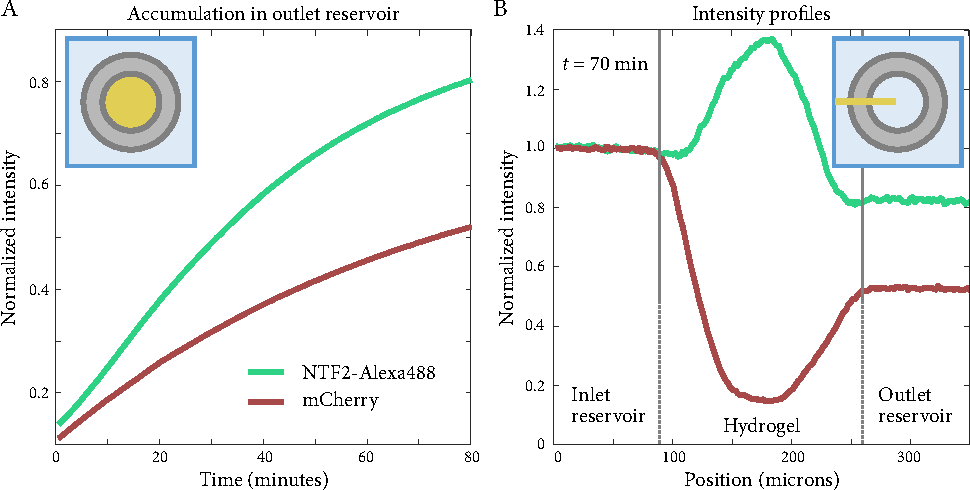
\includegraphics[width=0.7\textwidth]{figs/ch03/ring-acc-and-profile}
\label{fig:ring-acc-and-profile}
\end{figure} %16-08-19, chamber 1, #2 (1/32 dwell time, 2 loops) 

Confocal crosslinking does not damage FSFG, as demonstrated in Fig.~\ref{fig:LW-NTF2-images}.  Hydrogels were made using the precursor solution described above with the addition of 10 mg/mL FSFG-cys.  After soaking in PTB buffer overnight, a mixture of 25 $\mu$m each NTF2-Alexa488 and mCherry was added to the outer reservoir.  After two hours of equilibration, the FSFG hydrogels showed a partition coefficient greater than one for NTF2-Alexa488 but smaller than one for mCherry.  This indicates that FSFG is anchored into the gel and that NTF2-A488 is able to bind it.

Finally, Norland Optical Adhesive (NOA) can also be crosslinked using this method.  Complicated flow chambers can be created, although it is labor-intensive and difficult to remove all of the excess NOA afterwards.

\begin{figure} % LKM book 4 pg 57 (line); NEED TO FIND RING
\caption{Image of laser-written line FSFG hydrogel. 8/17/16}
\centering
%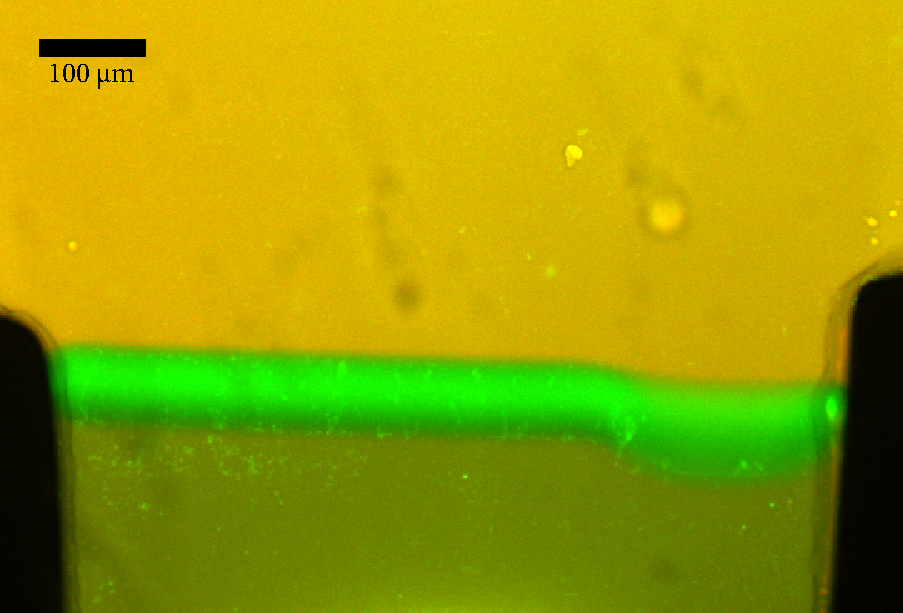
\includegraphics[width=0.5\textwidth]{figs/ch03/160817-bar-image-100umScale.pdf}
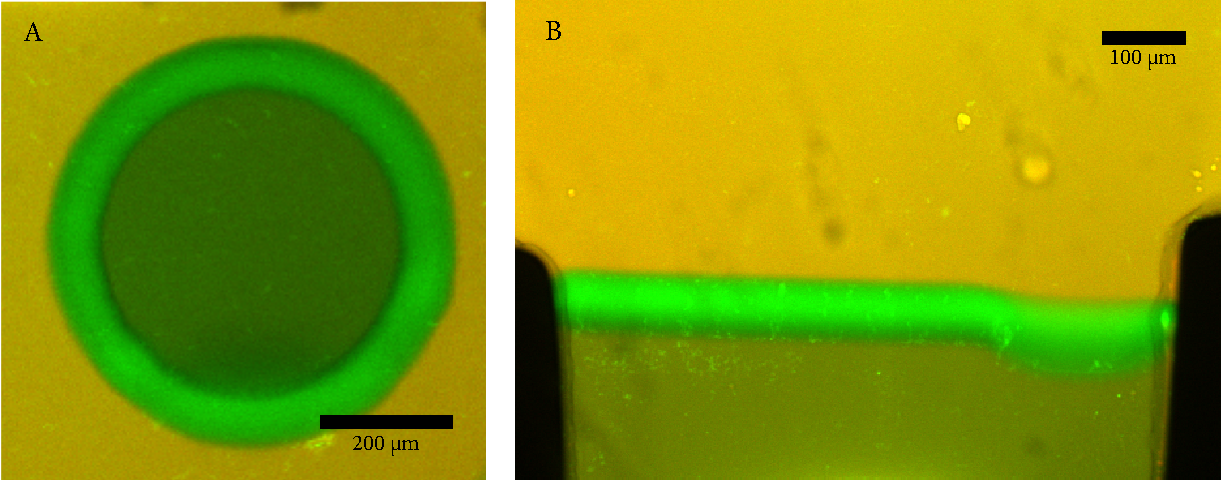
\includegraphics[width=0.8\textwidth]{figs/ch03/example-LW-gels-NTF2}
\label{fig:LW-NTF2-images}
\end{figure} % microscope settings for bar: 1/32 dwell, 2 loops, 100% photobleaching intensity, nominal thickness 50um, nominal concentration 50 mg/mL FSFG (slightly unclear? could be 10), 25 uM each NTF2-A488 and mCherry
% I am confused as to the date of the bar image.  Saved as 160817 in the microscopy folder so that's probably right

Despite the advantages of confocal crosslinking, several obstacles combined to ultimately make this method unusable for our purposes.  The most serious problem was that of stray crosslinking.  Areas outside of the defined region of interest were often unpredictably crosslinked, as can be seen in Fig.~\ref{fig:LW-gel-images}.  Stray crosslinking outside of the rings is limited by rinsing the gels within 5 minutes of crosslinking, removing any excess precursor solution \cite{paustian13}.  However, rinsing the chamber does not remove precursor solution from the ring's inner reservoir.  Stray crosslinking in this reservoir is often more difficult to detect and more damaging to the experimental results. Figure~\ref{fig:LW-NTF2-images} illustrates the problem: the ring has been equilibrated with NTF2-A488, which has preferentially entered the inner reservoir over mCherry.  The concentration of NTF2-A488 is, in fact, higher in the inner than the outer reservoir, indicating that there is some low concentration of FSFG available in the inner reservoir for binding to NTF2.  As the hydrogel was soaked in buffer overnight after crosslinking, any mobile FSFG remaining from the precursor solution has been removed, meaning that the remaining FSFG is most likely anchored into a lightly-crosslinked hydrogel that fills the inner reservoir.  The presence of this gel alters the results of an equilibration experiment by artificially increasing the final NTF2 concentration in the inner reservoir.

With help from Dani Konetski in Chris Bowman's group, I attempted to address the stray crosslinking by adding a photoinhibitor to the precursor solution.  The radical inhibitor 2,2,6,6-tetramethylpiperidine 1-oxyl (TEMPO) can be used in aqueous solution to limit crosslinking \cite{chatani14}.  I tested the effect of the photoinhibitor using a precursor solution as described above with the addition of 0.5 mM TEMPO.  While the edges of the resulting hydrogels became marginally sharper, stray crosslinking was still evident, especially in the inner reservoir.

%Help from Dani Konetski in Bowman lab with TEMPO and digital light projector (didn't work)
% TEMPO - LKM book 4 pgs 83-93

Another significant problem was swelling and buckling of the hydrogels.  Despite the hope that thinner hydrogels would swell and equilibrate more easily, buckling of the rings and lines was pervasive and difficult to predict (Fig.~\ref{fig:LW-gel-images}).  Ring hydrogels in particular often developed minor leaks due to buckling.  Despite a great many attempts to improve the swelling problem (see various other sections), the rings ultimately could not be used for selective transport experiments.

\begin{figure} % LKM book 4 pg 60
\caption{Comparison of edge dip for different dwell times, loop numbers}
\centering
\includegraphics[width=0.5\textwidth]{figs/ch03/dwell-time-effect}
\label{fig:dwell-time-effect}
\end{figure} %16-08-19, chamber 1, #2 (1/32 dwell time, 2 loops) compared to #6 (1 dwell time, 64 loops)

One interesting feature of confocal crosslinking is the degree of control it affords over the illumination method.  In the A1R's photobleaching mode, the 405 nm laser is raster-scanned over each pixel in the field of view.  The shutter is toggled in order to illuminate only pixels within the predefined region of interest.  The controls permit the laser intensity, dwell time at each pixel, and number of raster scan loops to be varied.  The laser intensity was always kept at 100\%, but changing the dwell time and loop number had a dramatic effect on the final properties of the hydrogel.

Generally speaking, a longer dwell time at each pixel and a low number of loops gave the best results.  (See if I can try to get dwell times in absolute time instead of fold change.)  Figure~\ref{fig:dwell-time-effect} shows post-equilibration profiles for two hydrogel rings made with different illumination settings.  Each gel received the same total illumination time, but in one case the dwell time was reduced 32-fold and the loop number increased by the same factor.  In both cases, the hydrogels were soaked in PTB buffer overnight and then challenged with 25 $\mu$M NTF2-Alexa488 and mCherry.  After 70 minutes, sufficient NTF2 had accumulated in the gel to make the differences between gels obvious.  The low-dwell-time hydrogel accumulated less NTF2 and displayed noticeable dips in NTF2 accumulation at both its inner and outer edges.  The edge-dip is reminiscent of those noted in the gels crosslinked by photomasking and the UV LED.  While the cause of the dip is unclear, it may be the result of diffusion of fresh precursor solution into the edge region over the course of the crosslinking process.  The fresh precursor then crosslinks, leading to a dense hydrogel edge that excludes NTF2 and mCherry.  This hypothesis is consistent with the observation that a longer dwell time and fewer raster loops largely eliminated the edge dip.  With fewer raster loops, there is less opportunity for diffusion of uncrosslinked precursor solution into the gel edge.  It should also be noted that the edge dip does not form when an entire droplet of precursor solution is crosslinked with the UV LED (i.e. no mask is used), further supporting the diffusion explanation.  In any case, long dwell times and low loop numbers are clearly preferable with confocal crosslinking.

In conclusion, confocal crosslinking has a number of advantages over LED crosslinking, and a corresponding number of obstacles.  Despite the attraction of testing selective transport using small hydrogel rings, we ultimately chose to use a much simpler hydrogel geometry and crosslinking method.

\section{Nup and transport factor constructs}
Figures
\begin{enumerate}
\item cartoon of various NTF2 constructs
\item table with FSFG variant sequences?
\item SDS-PAGE with FSFG cct2?
\end{enumerate}

\subsection{SSSG negative control}
The behavior of NTF2 and mCherry in FSFG hydrogels can be compared to that in hydrogels containing no Nups.  However, it is possible that the presence of FSFG in the precursor solution changes the final gel properties such as pore size, or that non-specific interactions between the Nup peptide and test proteins alter the behavior of the test proteins.  To account for these possibilities, we designed a negative control peptide which is identical to FSFG except that the phenylalanine residues have been mutated to serine, so that the binding motifs become SSSG.  This mutant does not bind NTF2, as demonstrated by the lack of NTF2 accumulation in hydrogels containing SSSG. Figure~\ref{fig:SSSG-control-comparison} compares the intensity profile of a 10 wt\% PEG hydrogel containing a nominal 10 mg/mL SSSG to that of a hydrogel with no nups.  There is no dramatic difference between the two profiles, suggesting that the presence of peptide in the hydrogel does not itself alter the diffusion of NTF2 and mCherry.  Following the initial tests, SSSG gels were used periodically to confirm that no-Nup gels served well as negative controls, but they were not used regularly as controls.

The SSSG peptide was used in an identical manner to FSFG: SSSG-cys was his-tagged, inserted into pRSF, and expressed in BL21-DE3 Gold cells.  It was purified using a cobalt affinity column using the same procedure as FSFG variants and had a high yield.  As with FSFG, SSSG is stable and non-aggregating over a wide range of conditions.
%I think Eric did most of the cloning work on this project and/or we bought the gene.
\begin{figure} % 6/9/15 for both SSSG and control (no-nup) gels, not sure whether or not I ran it personally, LKM book 2 pg 24
\caption{Comparison of intensity profiles for SSSG and no-nup (control) gels.}
\centering
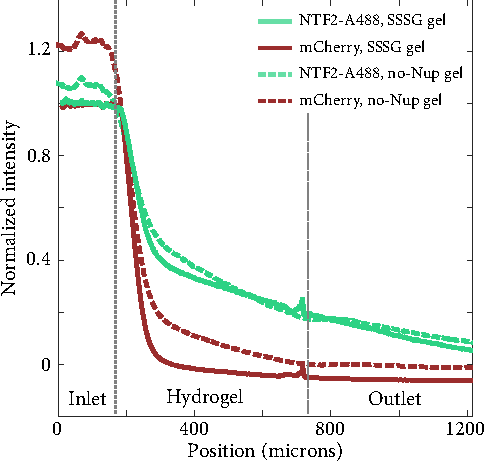
\includegraphics[width=0.8\textwidth]{figs/ch03/SSSG-control-comparison}
\label{fig:SSSG-control-comparison}
\end{figure} 
\subsection{Covalently-tethered NTF2 dimer}
One recurring problem we observed was that NTF2 moves faster in the hydrogels and equilibrates to a higher level than mCherry, even in SSSG gels or gels with no Nups.  This could be because NTF2 is dissociating into two monomers which are smaller and move faster than mCherry.  This shouldn't be happening, because the $K_D$ of mammalian NTF2 is about 1 $\mu$M \cite{chaillan-huntington01}, which should be about the same for our yeast NTF2.  However, to avoid this problem, we tried to make a covalently-tethered version of NTF2, consisting of two NTF2 monomers connected by a flexible amino-acid tether.  (Look up tether compositions and put in a table.)  We tried tethers of several lengths, including 15, 12, and smaller (look this up, it was a mutagenesis accident).  Unfortunately, the tether probably messed up the dimerization interface.  Look up whether we ever got these expressed and purified.  If so, they didn't bind.  Maybe show an SDS-PAGE gel for the purification and an accumulation plot/ picture to show they didn't bind. Eric and Scott did most of the cloning work on this project.
\begin{align*}
\mathrm{10aa-linker}&:&\mathrm{TSGSGSGSPG}\\
\mathrm{15aa-linker}&:&\mathrm{TSGSPRGSSGSGSPG}\\
\mathrm{18aa-linker}&:&\mathrm{TSPGLVSRGSGSGSGSPG}
\end{align*}
\subsection{NTF2-GFP}

Another reccuring problem was free dye in the NTF2 channel.  After dye-labeling (see next section), the dye slowly hydrolyzes and leaves the NTF2.  In an attempt to fix this problem, Eric Verbeke and I created a version of NTF2 tethered to GFP by a short linker.  

This construct is in the pET21 plasmid, his-tagged, and expressed in BL21-DE3 Gold cells.  It was purified using a cobalt affinity column in PTB and 1:1000 PIC and eluted with 250 mM imidazole, yielding ample protein with moderate degradation products.


\begin{figure} % GFP-NTF2 = 150917, GFP-NTF2x2 = 150928
\caption{Intensity profile for GFP-NTF2 and mCherry showing no binding to FSFG hydrogel.}
\centering
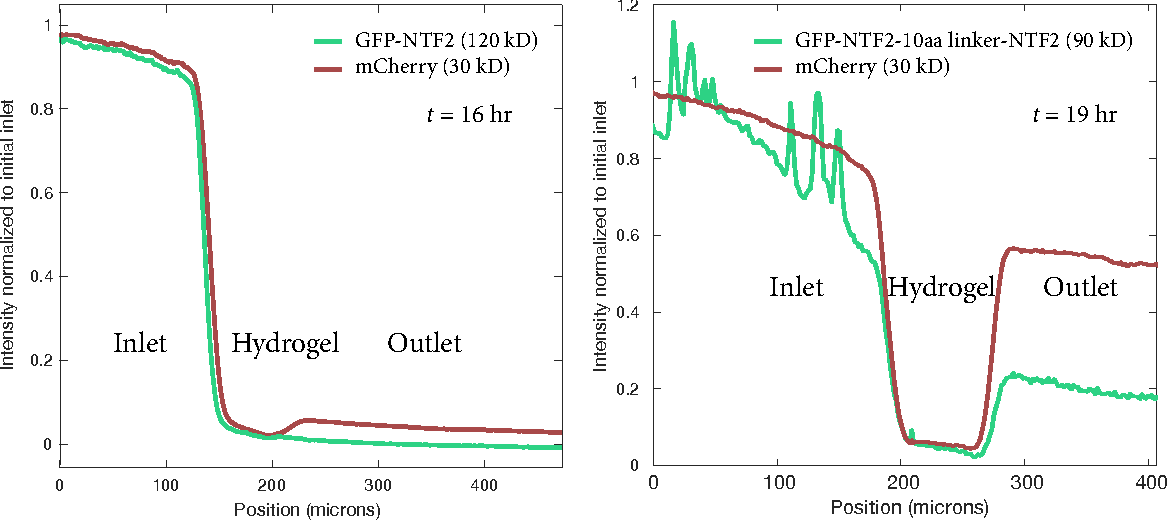
\includegraphics[width=\textwidth]{figs/ch03/GFP-NTF2-attempts.pdf}
\label{fig:GFP-NTF2}
\end{figure} 
\subsection{Covalently-tethered NTF2 dimer}

We were able to express and purify it, but it didn't bind to FSFG.  Probably the GFP was interfering with the binding site and/or dimerization interface?  

\subsection{Kap121 and NLS-GFP}
% Kap121 growth and purification - LKM book 2 pg 79, LKM book 3 pg 13, Chris Lawton book 1 pg 65, Loren's protocols in Google Drive, Jackie's paper
The karyopherins (Kaps) are a canonical class of transport factors.  They transport proteins tagged with nuclear localization signals (NLS) through the nuclear pore.  We were interested in testing Kaps because they are widely studied and much larger than NTF2, so selective transport would be more apparent.  Eric Verbeke engineered two GFP-NLS constructs: GFP-Spo12 and GFP-Pho4.  These constructs were his-tagged, inserted into pET21b, expressed in BL21-DE3 Gold cells, and purified using a cobalt affinity column. 
% GFP-NLS LKM book 2 pg 133
Kap121-GST was expressed and purified following \cite{tetenbaum-novatt12} and the GST subsequently cleaved with thrombin resin (Fig.~\ref{fig:Kap121}~a).
\begin{figure} % LKM book 4 pg 60
\caption{SDS-PAGE showing Kap121 purification (purified by Chris Lawton), picture of influx, intensity profiles}
\centering
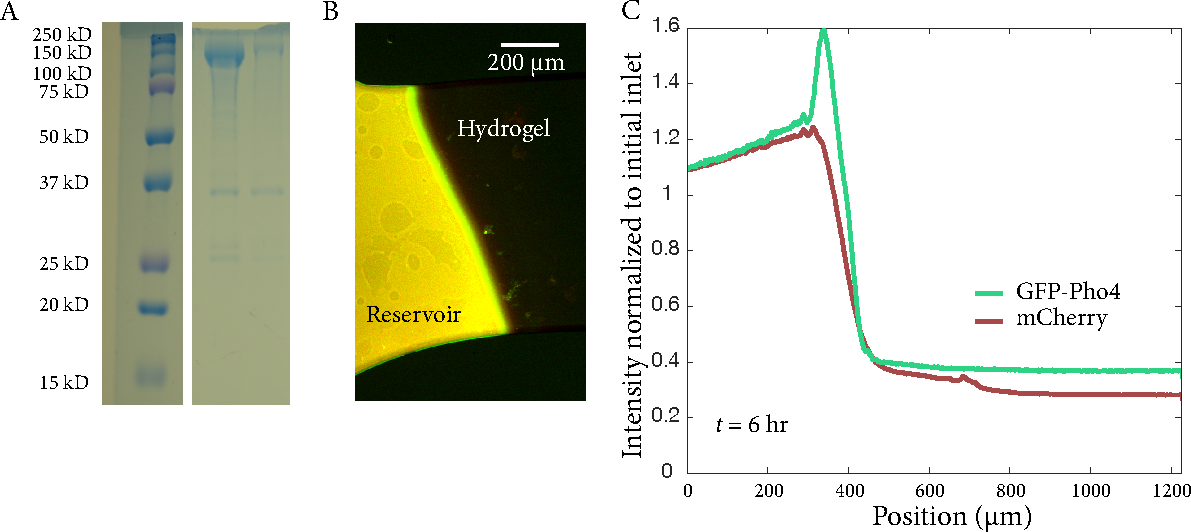
\includegraphics[width=\textwidth]{figs/ch03/Kap121}
\label{fig:Kap121}
\end{figure} % 12 polyacrylamide gel, 2hr, 100V, 10uL samples, purified by Chris Lawton, 5/28/15, saved in Laura's folder on lab desktop

% microscopy of Kap121 and Pho4 on 150602, LKM book 3 pg 19, used final frame of Kap121_Pho4 03 movie

Kap121 binding and influx was tested using a hydrogel made from precursor solution containing 0.05 wt\% Irgacure2959, 110 mg/mL 20kD 8-armed PEG-norbornene, 11 mg/mL 1kD PEG-dithiol, and 1 mM TCEP in PTB, crosslinked for 2 minutes under the UV LED.  After soaking in PTB overnight, 5 $\mu$M Kap121, 10 $\mu$M GFP-Pho4, and 100 $\mu$M mCherry in PTB were added to the inlet reservoir.  Selective influx of the Kap121/GFP-Pho4 complex was evident, since the complex accumulated at the edge of the hydrogel (Fig.~\ref{fig:Kap121}~b and~c).  The bright band demonstrates binding of FSFG to Kap121 as well as of Kap121 to GFP-Pho4.  Over the course of several hours, the GFP front remained localized at the edge of the gel, likely indicating that the pore size of the hydrogel was too small to accomodate the Kap121/GFP-Pho4 complex.  Given the large size of this complex, the pore size was never increased sufficiently for influx into the hydrogels.

 % same as 110 mg/mL 20kD 8-armed PEG-norbornene, 11 mg/mL 1kD PEG-dithiol, and 1 mM TCEP in PTB;
%same as 10 wt% PEG, 0.5 thiol:ene ratio (LKM book 2 pg 73)

\subsection{FSFG concat 2 and concat 3}
In order to test the effect of Nup length and number of binding sites, we used multiple versions of FSFG.  We got these versions from Loren's old lab and didn't really modify them.  Eric may have added a cysteine for labeling.  FSFG concat 2 is twice as long, and FSFG concat 3 is three times as long.  Maybe I should include sequences of all three FSFG variants.  Both variants express in principle, but I could only get FSFG concat 2 to express.  I purify it using the same method as FSFG concat 1 (the original form, with 124 amino acids and 6 FSFG repeats).  

\section{Dye-labeling and free dye}
% matlab results are saved in /Volumes/houghgrp/Old Processed Images/Old Analysis/FSFG dataset/exponent-fits.mat
Figures
\begin{enumerate}
\item Typhoon image of dye, Matlab peaks
\item Example of single- and double- exponential fits
\item goodness of fit measurements for single- and double- exponential fits
\end{enumerate}
We have to label NTF2 with a fluorescent dye to use it as a test transport factor.  For the most part, we've used Alexa Fluor 488 as the dye.  (Most recently we switched to fluorescein because it's easier to photobleach.)  There are several choices of labeling chemistry.  We've used both NHS and SDP esters, which label the exposed lysines of NTF2, of which there are several.  We've also tried using Alexa488-maleimide to label the cysteine of an engineered NTF2-cys.  Both labeling chemistries result in bonds that eventually hydrolyze, cleaving the dye from the protein.  This is a major problem for the experiments, since free dye (about 1kD) diffuses much faster than dye bound to a protein and is experimentally identical.  Non-negligible levels of free dye would give the impression that NTF2 is equilibrating significantly faster than it actually is.  The maleimide-labeling chemistry is more stable, but in practice not as efficient as the ester-labeling protocol.  It also requires using NTF2-cys, which could introduce other issues.  Mostly I stuck with the lysine-labeling protocol, which needed significant optimization to minimize free dye issues.  Eric did a lot of work in optimizing the cysteine-labeling protocol, and I took his work as a base in optimizing the lysine-labeling protocol.

-list cysteine labeling protocol here
-list lysine labeling protocol here

\subsection{Labeling NTF2 with fluorescein-NHS}
\begin{enumerate}
\item Resuspend lyophilized fluorescein-NHS at 100 mg/mL in anhydrous DMSO in the darkroom.  Discard the remaining DMSO aliquot.  Make 100-$\mu$L aliquots of dye solution. Store with desiccant in ultra-low freezer, protected from light.
\item Mix NTF2 in PTB pH 7.0 and 100 mg/mL fluorescein-NHS in DMSO with around 15-fold molar excess dye.  Several other buffers can be used as well (see Thermo protocol).  A typical labeling reaction used 0.5 mL of 16 mg/mL NTF2 and 18.6 $\mu$L dye stock mixed in an Eppendorf with an Eppendorf stir bar.
\item Incubate mixture, stirring, protected from light, at room temperature for one hour.
\item Equilibrate TALON cobalt resin with PTB in a column that can be spun in a centrifuge.  TALON resin has a stated capacity of 5-15 mL protein per mL resin.  Using significantly more than needed can lead to nonspecfic binding of free dye.  A typical reaction required 1.6 mL of the resin slurry.  Equilibrate with at least 10 bed volumes PTB.
\item Cap column and add reaction mixture.  Nutate at 4$^\circ$C for one hour, protected from light.
\item Allow column to drain and wash with approximately 100 bed volumes of PTB, protected from light as best as possible.  Occasionally cap column and resuspend resin to remove free dye from column cap and sides.  Test flow-through using UV light to ensure that no dye is visible by the end of the wash.  Resin should still be bright yellow.
\item Spin column 1000 rpm (convert to rpm, spun in 15 mL conical) for one minute to remove remaining wash buffer.  Immediately cap and elute with 1 mL of 300 mM imidazole in PTB.  Nutate 4$^\circ$C for half an hour and collect elution.  Resin should return to pink.
\item Dialyze elution against PTB to remove imidazole.  No more than 24 hours after labeling, aliquot and freeze labeled NTF2.
\item Run a sample of labeled NTF2 on a native PAGE gel along with a sample of fluorescein-NHS.  Use the Typhoon to compare the concentration of free dye to labeled protein in the protein sample.
\end{enumerate}
\subsection{Labeling NTF2 with Alexa Fluor 488 - SDP}
\begin{enumerate}
\item Resuspend lyophilized Alexa Fluor 488 at 10 mg/mL in anhydrous DMSO in the darkroom.  Discard the remaining DMSO aliquot.  Make 10-$\mu$L aliquots of dye solution. Store with desiccant in ultra-low freezer, protected from light.
\item Mix NTF2 in 0.1 M sodium bicarbonate buffer and 10 mg/mL fluorescein-NHS in DMSO with around ??-fold molar excess dye.  A typical labeling reaction used 200 $\mu$L of 16 mg/mL NTF2 and 20 $\mu$L dye stock mixed in an Eppendorf with an Eppendorf stir bar.
\item Incubate mixture, stirring, protected from light, at room temperature for one hour.
\item Equilibrate TALON cobalt resin with PTB in a column that can be spun in a centrifuge.  TALON resin has a stated capacity of 5-15 mL protein per mL resin.  Using significantly more than needed can lead to nonspecfic binding of free dye.  Equilibrate with at least 10 bed volumes PTB.
\item Cap column and add reaction mixture.  Nutate at 4$^\circ$C for one hour, protected from light.
\item Allow column to drain and wash with approximately 100 bed volumes of PTB, protected from light as best as possible.  Occasionally cap column and resuspend resin to remove free dye from column cap and sides.  Test flow-through using UV light to ensure that no dye is visible by the end of the wash.  Resin should still be bright yellow.
\item Spin column 500 rpm (convert to rpm, spun in mini centrifuge) for 20 s to remove remaining wash buffer.  Immediately cap and elute with 300 $\mu$L of 500 mM imidazole in PTB.  Nutate 4$^\circ$C for half an hour and collect elution.  Resin should return to pink.
\item Dialyze elution against PTB to remove imidazole.  No more than 24 hours after labeling, aliquot and freeze labeled NTF2.
\item Run a sample of labeled NTF2 on a native PAGE gel along with a sample of fluorescein-NHS.  Use the Typhoon to compare the concentration of free dye to labeled protein in the protein sample.
\end{enumerate}
\subsection{Labeling NTF2-cys or FSFG-cys with Alexa Fluor 488 - maleimide}
\begin{enumerate}
\item Resuspend lyophilized Alexa Fluor 488 at 10 mg/mL in anhydrous DMSO in the darkroom.  Discard the remaining DMSO aliquot.  Make 10-$\mu$L aliquots of dye solution. Store with desiccant in ultra-low freezer, protected from light.
\item Mix protein in PTB pH 7.0 and 50 $\mu$M TCEP (with no other reducing agent present) and 10 mg/mL dye in DMSO.  Check molar ratios, pg 70 LKM book 5.
\item Incubate mixture, stirring, protected from light, at room temperature for two hours.
\item Equilibrate TALON cobalt resin with PTB in a column that can be spun in a centrifuge.  TALON resin has a stated capacity of 5-15 mL protein per mL resin.  Using significantly more than needed can lead to nonspecfic binding of free dye.  Equilibrate with at least 10 bed volumes PTB.
\item Cap column and add reaction mixture.  Nutate at 4$^\circ$C for one hour, protected from light.
\item Allow column to drain and wash with approximately 100 bed volumes of PTB, protected from light as best as possible.  Occasionally cap column and resuspend resin to remove free dye from column cap and sides.  Test flow-through using UV light to ensure that no dye is visible by the end of the wash.  Resin should still be bright yellow.
\item Spin column 500 rpm (convert to rpm, spun in mini centrifuge) for 20 s to remove remaining wash buffer.  Immediately cap and elute with 300 $\mu$L of 500 mM imidazole in PTB.  Nutate 4$^\circ$C for half an hour and collect elution.  Resin should return to pink.
\item Dialyze elution against PTB to remove imidazole.  No more than 24 hours after labeling, aliquot and freeze labeled NTF2.
\item Run a sample of labeled NTF2 on a native PAGE gel along with a sample of fluorescein-NHS.  Use the Typhoon to compare the concentration of free dye to labeled protein in the protein sample.



0.1 M sodium bicarbonate buffer and 10 mg/mL fluorescein-NHS in DMSO with around ??-fold molar excess dye.  A typical labeling reaction used 200 $\mu$L of 16 mg/mL NTF2 and 20 $\mu$L dye stock mixed in an Eppendorf with an Eppendorf stir bar.
\end{enumerate}

The major change is the increased wash step, and the immediate aliquoting and freezing before use.  I also began to be much more careful with characterizing the results of the labeling.  Immediately after finishing dialysis, I run a BCA to quantify the protein concentration in the labeled sample.  The same day, I aliquot and freeze all the protein except a sample for the remaining tests.  As soon as possible, I run a native PAGE gel, including the labeled protein sample as well as a free dye sample.  After running the gel, I image it in the Alexa488 channel using the Typhoon, and then stain with Coomassie to make sure the protein hasn't degraded.  I use Matlab to compare the amplitude of the labeled-protein band and the free-dye band that remains in the labeled-protein sample.  Typically, the free dye band is 1-3\% the amplitude of the labeled-protein band.  Finally, I measure the absorbance of the labeled protein at 494 (check this wavelength) nm and use Beer's law to find the concentration of Alexa488.  I can compare this measurement with the protein measurement from the BCA to calculate a labeling efficiency.  Include some sample efficiencies here.  I typically get lower efficiencies than other people report.  I spoke to Annette and she had no major suggestions.  In principle, doing the reaction under nitrogen would help, but Annette gets something like 90\% efficiency without doing that.  I use the labeled NTF2 immediately after thawing if possible, and no more than a week after thawing.

We also tried to make NTF2-GFP to fix the free dye problem (see section above).

In addition to the tests I run on each batch of labeled NTF2, at one point I did some mathematical analysis to confirm that the free dye was only a minor problem in the experiments I had already run.  In order to confirm that, I fit the accumulation curves to single or double exponentials (they really should have been erfc functions but I approximated.)
%%%%

If there is no free dye, as in the case of the mCherry accumulation, the accumulated intensity $I(t)$ can be approximated as
\begin{equation}
I(t) = A_1\exp(-t/\tau_1) +C
\label{eq:single-exp}
\end{equation}
with some amplitude $A_1$, equilibration lifetime $\tau_1$, and constant offset $C$.  In this case, a non-zero value of $C$ is likely due to background fluorescence.  If, on the other hand, a sample contains a population of small, free dye molecules as well as large labeled protein, both populations will equilibrate at different rates, leading to an accumulated intensity of
\begin{equation}
I(t) = A_1\exp(-t/\tau_1) + A_2\exp(-t/\tau_2)+C
\label{eq:double-exp}
\end{equation}
where each population has an equilibration lifetime as well as an amplitude related to its abundance in the sample.

I fit a collection of 43 accumulation experiments to both Eqns.~\ref{eq:single-exp} and \ref{eq:double-exp}.  I compared the resulting parameters as well as the adjusted R-square value of each fit.  Adding more parameters to the fit will always improve the fit, but the adjusted R-square is intended to account for the effect of adding more parameters to a model.  A higher adjusted R-square therefore means a better fit.

The mCherry accumulation fits did not noticeably improve when moving from the single to the double exponential.  In addition, the lifetimes and amplitudes of each component of the two-component fit were apparently uncorrelated.  Both results support the fact that there is no free dye in the red channel, since the only fluorescence is coming from mCherry.

On the other hand, the NTF2 fits did result in a higher adjusted R-square value on average with the double-exponential fit.  Strikingly, the two components sorted themselves into two categories: a low-amplitude, short-lifetime component and a high-amplitude, long-lifetime one.  The most straightforward interpretation is that the low-amplitude component is the free dye, which should be present in  low amounts and equilibrate much more rapidly than labeled protein, thanks to its small size.

The median amplitude of the free-dye signal was 1.2\% that of the labeled-protein signal, using a sample of 43 experiments.  The median free-dye equilibration lifetime was 50 minutes, as compared to approximately 2000 minutes for the labeled-protein lifetime.  These results confirm that the new, more stringent dye-labeling protocol is successful in removing almost all free dye from the labeled-protein sample, and that the hydrolysis of the dye is negligible on the time scale of the experiment and enforced shelf life of the labeled protein.

Also made GFP-NTF2 (didn’t bind to FSFG)


